\documentclass[12pt]{article}
\everymath{\displaystyle}
\usepackage{unicode-math}
\usepackage{pgfplots}
\pgfplotsset{compat=1.18}
\usepackage{amsmath}



\usepackage[margin=1in]{geometry}
\usepackage{tcolorbox}
\usepackage{graphicx}
\usepackage{tikz}
\usepackage{amssymb}
\usepackage{enumitem}
\usepackage{titlesec}
\usepackage{fancyhdr}
\usepackage{pifont}
\usepackage{xcolor}
\newcounter{questionnum}
\setcounter{questionnum}{0}
\usepackage{eso-pic} % for page background

% --------- 主题颜色设置 ---------
\definecolor{novelblue}{RGB}{70,60,150}
\definecolor{headerbg}{RGB}{240,240,255}

\pagestyle{fancy}
\fancyhf{}
\renewcommand{\headrulewidth}{0.4pt}
\renewcommand{\headrule}{\hbox to\headwidth{\color{novelblue}\leaders\hrule height 0.4pt\hfill}}

% --------- 页眉背景色条 ---------
\newcommand{\headbackground}{
  \AddToShipoutPictureBG*{
    \begin{tikzpicture}[remember picture, overlay]
      \fill[blue!5!purple!10] (current page.north west) rectangle ([yshift=-60pt]current page.north east);
    \end{tikzpicture}
  }
}

% --------- 页眉设置 ---------
\pagestyle{fancy}
\fancyhf{}
\renewcommand{\headrulewidth}{0pt}
\fancyhead[L]{\color{novelblue}\textbf{\textbf{Novel Prep} }}
\fancyhead[C]{\color{novelblue}\textbf {SAT Preparation}}
\fancyhead[R]{\color{novelblue}\textbf{Jack Zeng}}


\newtcolorbox{SATCard}[1][]{%
  enhanced,
  colback=white,
  colframe=novelblue,
  coltitle=white,
  boxrule=0.6pt,
  arc=4pt,
  boxsep=5pt,
  left=8pt, right=8pt, top=10pt, bottom=10pt,
  sharp corners=south,
  drop shadow south east,
  #1
}

% --------- 顶部 Mark for Review 栏 ---------
\newcommand{\markforreview}{
  \stepcounter{questionnum} % 自动递增题号
  \begin{tikzpicture}[scale=1.1]
    % 黑色题号
    \fill[black] (0,0) rectangle (0.8,0.6);
    \node[white, font=\bfseries\large] at (0.4,0.3) {\thequestionnum};

    % 灰底主栏
    \fill[gray!10] (0.8,0) rectangle (14.5,0.6);

    % Mark for Review
    \node[anchor=west, font=\small] at (1.2,0.3) {\ding{72} \hspace{2pt}Mark for Review};

    % ABC 按钮区域
    \draw[thick, rounded corners=3pt] (13.5,0.12) rectangle (14.5,0.48);
    \node[font=\bfseries\normalsize] at (14.0,0.3) {ABC};
  \end{tikzpicture}


  \newcommand{\choiceboxcircled}[2]{%
  \begin{tcolorbox}[
    colback=white,
    colframe=black,
    boxrule=0.5pt,
    rounded corners=6pt,
    left=6pt, right=6pt, top=6pt, bottom=6pt,
    width=\linewidth
  ]
    \textbf{\large\textcircled{\textbf{#1}}} \ #2
  \end{tcolorbox}
}
}

% --------- 选项框样式 ---------
\newcommand{\choicebox}[2]{%
  \begin{tcolorbox}[
    colback=white, 
    colframe=novelblue,
    boxrule=0.5pt, 
    rounded corners=4pt, 
    left=6pt, right=6pt, top=6pt, bottom=6pt,
    width=\linewidth
  ]
  \textbf{#1.} \ #2
  \end{tcolorbox}
}


\begin{document}
\section*{Math Hard Question 9}
\noindent\markforreview
\vspace{1em}

Elizabeth has \$4500 in an account.  
Each year she expects to have **11\% more** money in the account than the previous year.  
Which of the following models best describes how Elizabeth expects the money in her account to change over time?

\choicebox{A}{Decreasing exponential}  
\choicebox{B}{Decreasing linear}  
\choicebox{C}{Increasing exponential}  
\choicebox{D}{Increasing linear}

\vspace{2em}

\noindent\markforreview
\vspace{1em}

The function  
\[
T(x) = \frac{20{,}000 - 6.5x}{1{,}000}
\]  
gives the estimated air temperature \(T(x)\), in degrees Celsius (\(^\circ\)C), at an altitude of \(x\) meters.  

If the estimated temperature surrounding the hot air balloon is **15°C**,  
which of the following is closest to the altitude \(x\) of the hot air balloon?

\choicebox{A}{20}  
\choicebox{B}{769}  
\choicebox{C}{1,333}  
\choicebox{D}{5,385}

\newpage
\noindent\markforreview
\vspace{1em}

The function \(f\) is defined as:  
\[
f(x) = (x - a)(x - b)
\]  
where \(a\) and \(b\) are integer constants.  

Given that:  
\(f(17) > 0,\quad f(20) < 0,\quad f(23) > 0\)  

What is one possible value of \(a + b\)?

\choicebox{A}{39}  
\choicebox{B}{38}  
\choicebox{C}{37}  
\choicebox{D}{36}

\vspace{2em}
\noindent\markforreview
\vspace{1em}

The positive number \(a\) is 2,106\% of the sum of the positive numbers \(b\) and \(c\),  
and \(b\) is 81\% of \(c\).  

What percent of \(b\) is \(a\)?

\choicebox{A}{4,706\%}  
\choicebox{B}{47.06\%}  
\choicebox{C}{470600\%}  
\choicebox{D}{47060\%}

\newpage

\noindent\markforreview
\vspace{1em}

For the function \(f\), for every increase of 2 in the value of \(x\),  
the value of \(f(x)\) increases by a factor of \(c\), where \(c\) is a constant.  

Which of the following equivalent forms of function \(f\) displays the value of \(c\)  
as the base or the coefficient?

\choicebox{A}{\(f(x) = 42(2)^6\)}  
\choicebox{B}{\(f(x) = 42(8)^2\)}  
\choicebox{C}{\(f(x) = 42(64)^x\)}  
\choicebox{D}{\(f(x) = 42(4096)^{\frac{x}{2}}\)}


\vspace{2em}
\noindent\markforreview
\vspace{1em}

A study investigated the effect of magnesium supplementation on sleep quality.  
190 adults were randomly selected, and their sleep efficiency was measured.  

Participants were randomly assigned to take a magnesium supplement or a placebo for 6 weeks.  
The study concluded that magnesium improved sleep quality.  

What feature of this study supports this conclusion?

\choicebox{A}{There were more than 100 participants in the study.}  
\choicebox{B}{The participants were selected at random from the community center.}  
\choicebox{C}{The sleep efficiency of each participant was measured again at the end of 6 weeks.}  
\choicebox{D}{Each participant was randomly assigned to take a magnesium supplement or a placebo.}

\newpage
\noindent\markforreview
\vspace{1em}

A circle in the \(xy\)-plane has its center at \((-1, 1)\).  
Line \(t\) is tangent to this circle at the point \((7, -6)\).  

Which of the following points also lies on line \(t\)?

\choicebox{A}{(0, 7)}  
\choicebox{B}{(6, 9)}  
\choicebox{C}{(14, 2)}  
\choicebox{D}{(15, 1)}

\vspace{2em}

\noindent\markforreview
\vspace{1em}

The function \(f(x)\) is defined by:  
\[
f(x) = \frac{x^2 + ax + b}{2x + c}
\]  
where \(a\), \(b\), and \(c\) are constants.  

The graph of \(f(x)\) does not intersect the line \(x = 4\).  
If \(f(5) = f(6) = 0\), what is the value of \(a + b + c\)?

\choicebox{A}{10}  
\choicebox{B}{11}  
\choicebox{C}{12}  
\choicebox{D}{13}

\newpage

\noindent\markforreview
\vspace{1em}

    \begin{center}
        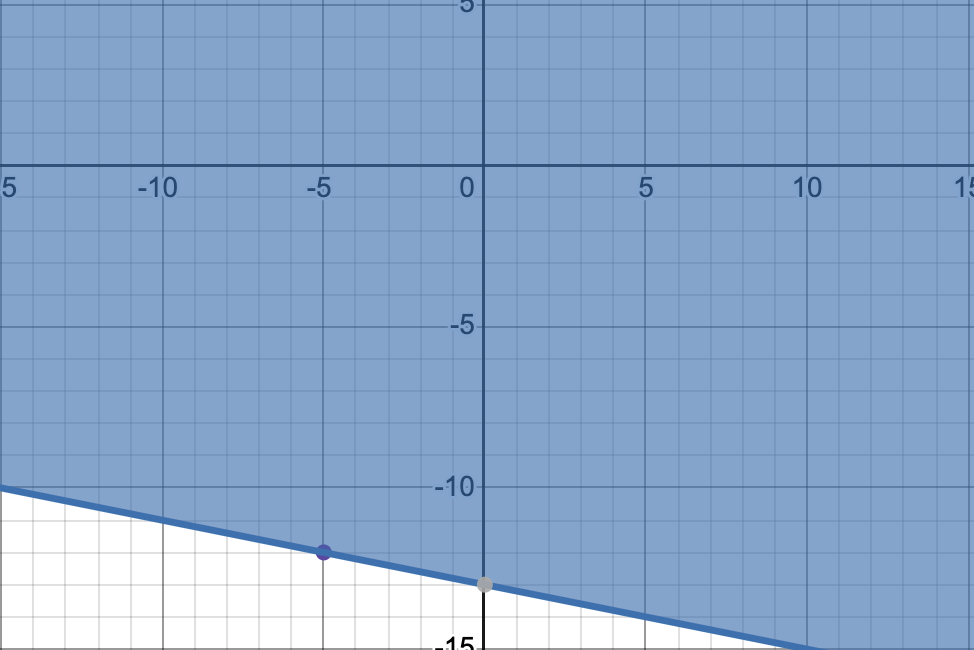
\includegraphics[width=0.6\linewidth]{f7.png}
    \end{center}


The shaded region represents the solutions to the inequality:  
\[
rx + ty \geq -65
\]  
What is the value of \(r + t\)?

\choicebox{A}{6}  
\choicebox{B}{4}  
\choicebox{C}{-4}  
\choicebox{D}{-5}

\vspace{2em}












\end{document}